\documentclass[10pt,twocolumn]{article}

% use the oxycomps style file
\usepackage{oxycomps}
\usepackage{listings}
\usepackage{graphicx}

% usage: \fixme[comments describing issue]{text to be fixed}
% define \fixme as not doing anything special
\newcommand{\fixme}[2][]{#2}
% overwrite it so it shows up as red
\renewcommand{\fixme}[2][]{\textcolor{red}{#2}}
% overwrite it again so related text shows as footnotes
%\renewcommand{\fixme}[2][]{\textcolor{red}{#2\footnote{#1}}}

% read references.bib for the bibtex data
\bibliography{references}

% include metadata in the generated pdf file
\pdfinfo{
    /Title (The Occidental Computer Science Comprehensive Project: Goals, Timeline, Format, and Advice)
    /Author (Justin Li)
}

% set the title and author information
\title{HTML Tutorial for Computer Science Students:\\
Junior Comps Tutorial Assignment 2}
\author{Charlie Rui Chai}
\affiliation{Occidental College}
\email{rchai@oxy.edu}

\begin{document}

\maketitle

\section{Introduction}
For my Comps Project, I want to build a dining review platform for the Occidental College community. This goal includes developing a web application and running it on a server. This tutorial will guide the reader through the process of building a webpage for restaurant menus on their local server. Restaurant menus are the essential elements of a dining review platform and is one of our main functionalities. We use HTML, CSS and JavaScript as programming languages, and run the webpage on google Chrome using VSCode Live Server extension. This tutorial aims to teach our readers the basics of web development skills and allow them to modify and build their own. In the future, we will learn more advanced skills such as Ajax to asynchronously update webpage content, and the React library to develop more efficient webpages.

\section{Methods}

To get started, we first install the development environment. We download Visual Studio Code (VSCode) from its website https://code.visualstudio.com. The Live Server extension was installed from VSCode “extensions market” to enable real-time preview of the webpage during the coding process, which simplifies debugging and testing. 

For the text and image content, we create a new HTML file and name it Menu.html. HTML is a markup language. It provides a means to create structured documents by denoting structural semantics for text such as headings, paragraphs, lists, links, quotes, and other items. We build a simple but typical layout for the menu page. The HTML file includes a main menu section with div containers for each menu item with appropriate class attributes for CSS styling. Each item within the menu is represented by an article tag, including details such as the item’s image, name, price, and description. 

To enhance the visual appeal of the webpage, we employ CSS to design visual effects for our webpage. Cascading Style Sheets (CSS) is a style sheet language used for specifying the presentation and styling of a document written in a markup language such as HTML or XML. The CSS file we use (styles.css) is provided by the tutorial repository. It contains global and menu styles with predefined font sizes, colors, borders, and other style variables.

The JavaScript file handles the logic of our webpage and is thus the main focus of the tutorial. To allow interaction between JS and HTML/CSS, we should first understand the Document Object Model (DOM). The DOM is a programming interface for web documents. The DOM represents the document as nodes and objects; that way, programming languages can interact with the page. In our tutorial, an example is the DOM specifies two method in this code snippet, which returns the first or all element within the document that matches the specified selector.

\begin{lstlisting}[caption= Document method example]
const sectionCenter = document.querySelector(".section-center");
const filterBtns = document.querySelectorAll(".filter-btn");
\end{lstlisting}

We also need to learn some useful Web APIs. To realize the buttons’ functionalities, we use the event listener to “listen” to events like users’ click on the button and do something after that. The addEventListener() method of the EventTarget interface sets up a function that will be called whenever the specified event is delivered to the target.

\begin{lstlisting}[caption= Listeners example]
filterBtns.forEach(function (btn) {
  btn.addEventListener("click", function (e) {
    console.log(e.currentTarget.dataset);
    const category = e.currentTarget.dataset.id;    
  })
})
\end{lstlisting}

We also need to learn to use functions, the fundamental building blocks in JavaScript. For students with Java experiences, function in JS is similar to function in Java. You must define it somewhere in the scope from which you wish to call it, and it will take some input and return an output. You don’t necessarily need to name the function or pass in an input.

For the actual JS code, we first initialize element selectors and event listeners as taught above. To load the content, we write a function that handles display menu items, and call it as soon as the webpage content is loaded. Now we have a static webpage, we want to add filtering features that navigate users to different types of cuisines. We write a function that generates filter buttons based on the categories available in the menu items. To allow filtering, we write the filter logic as shown. Following this tutorial, you should be able to build a similar webpage.


  \begin{figure}[h]
  \centering
  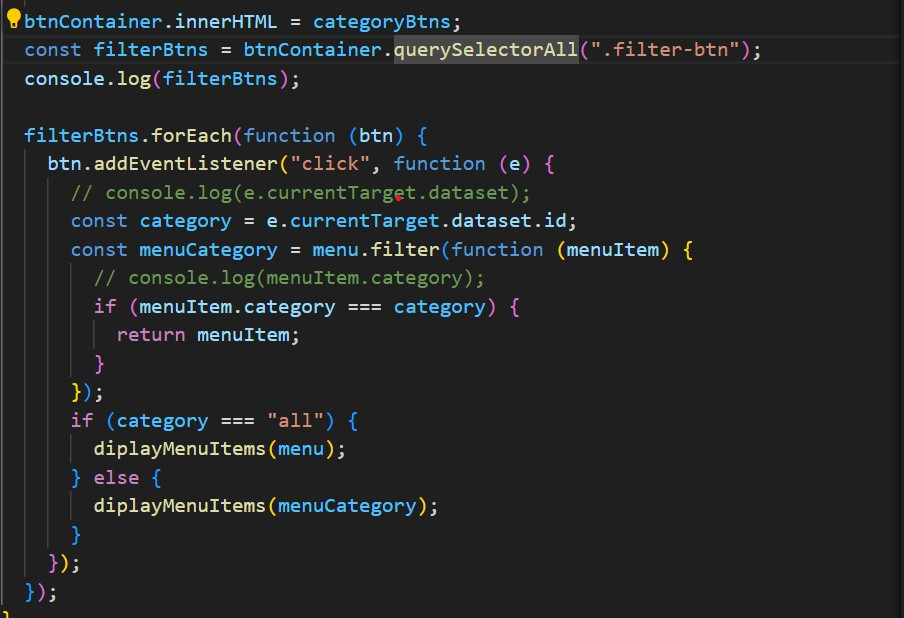
\includegraphics[width=0.45\textwidth]{Filter.jpg}
  \caption{Sample code for filter functionality.}
  \label{fig:image1}
\end{figure}

  \begin{figure}[h]
  \centering
  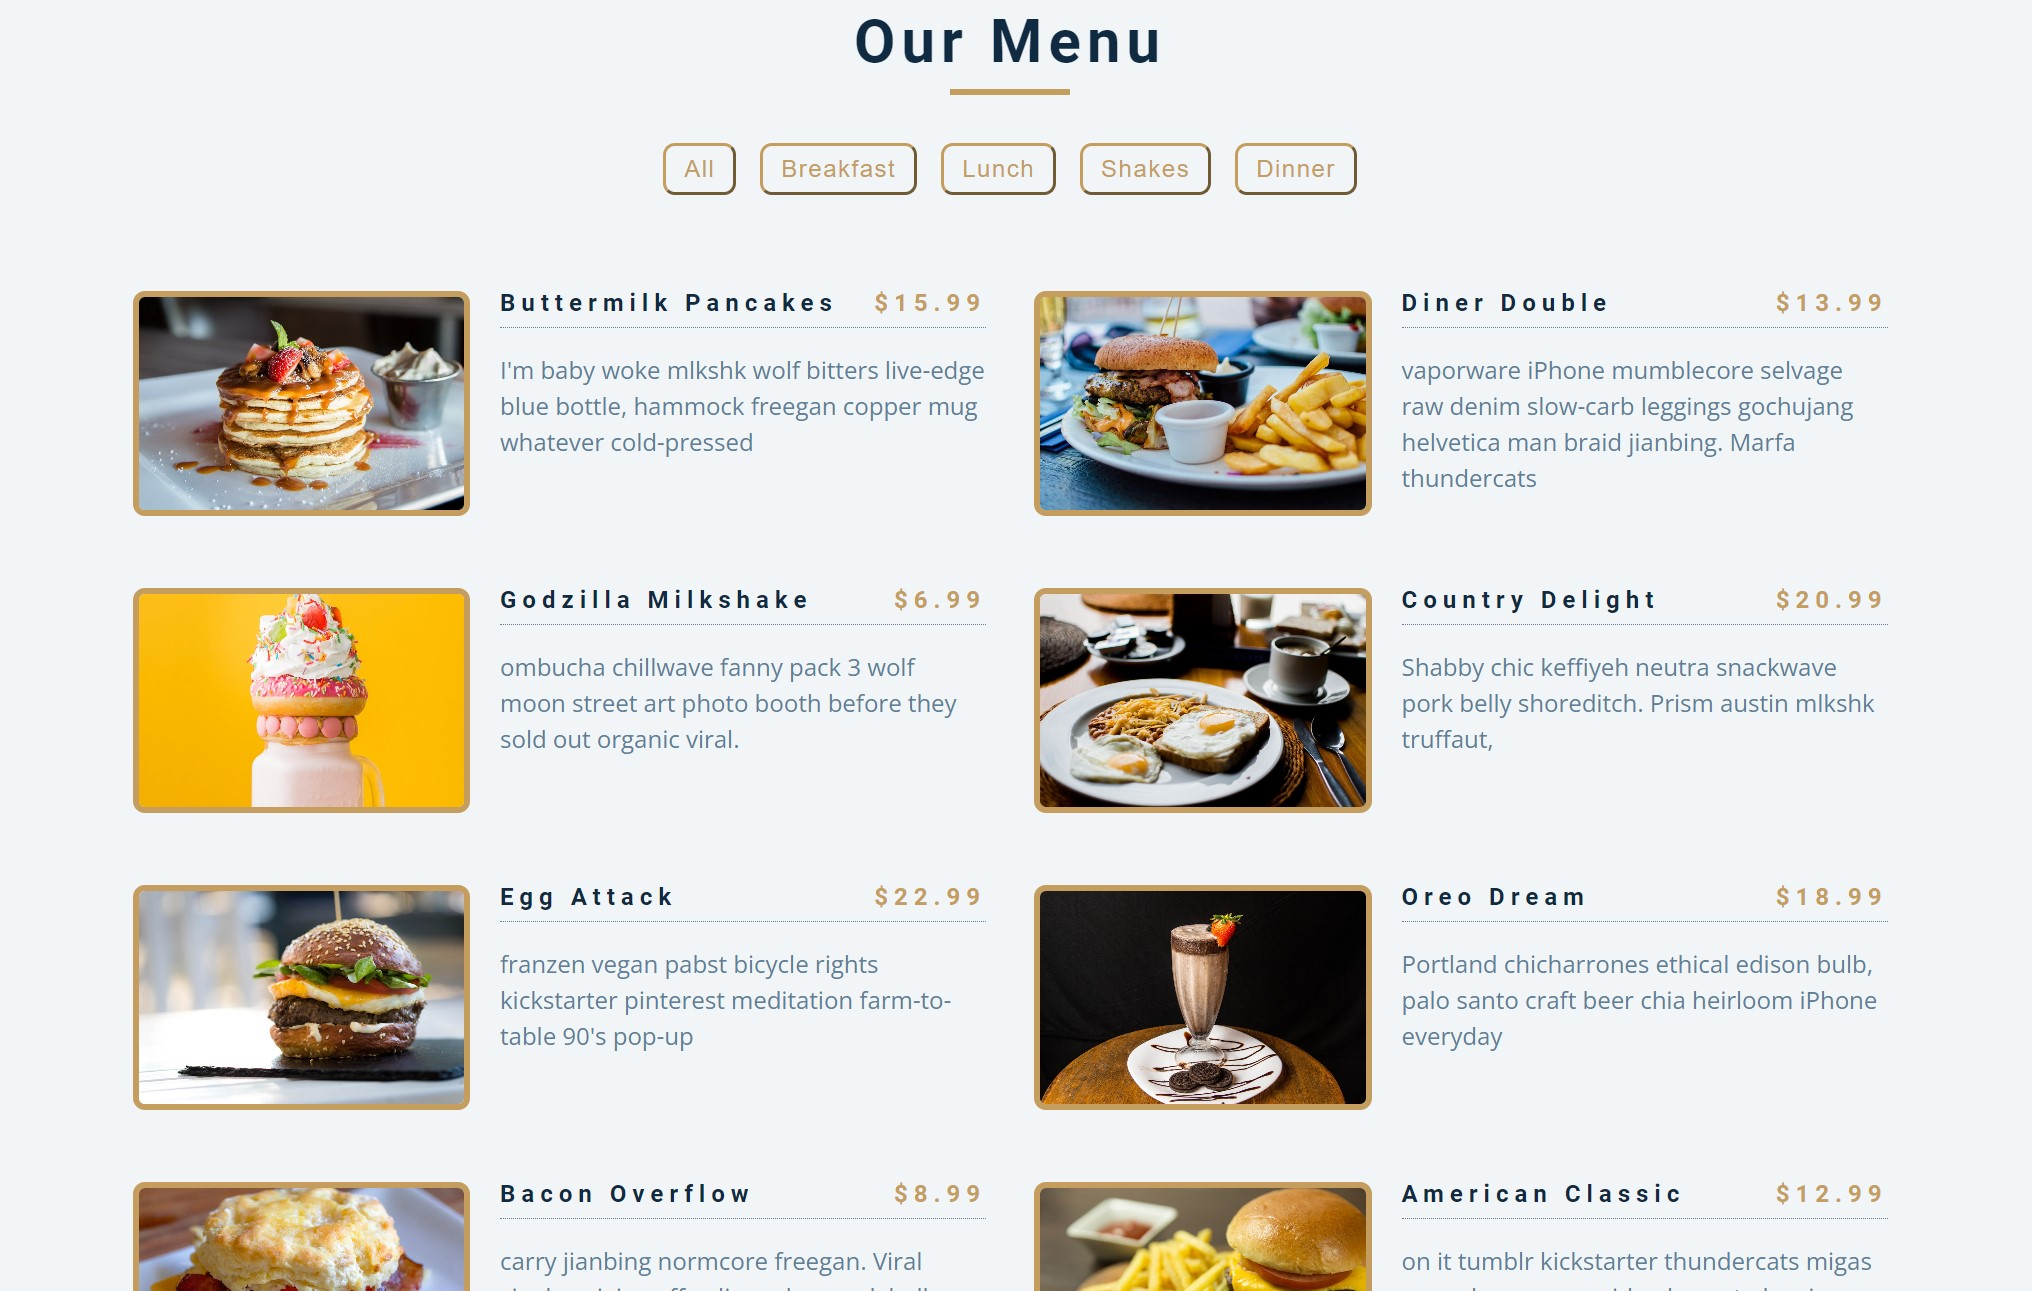
\includegraphics[width=0.45\textwidth]{Webpage.jpg}
  \caption{Sample Webpage.}
  \label{fig:image1}
\end{figure}



\section{Metrics and Results}

The primary goal of this tutorial was to build a dynamic and interactive webpage displaying and filtering a restaurant menu according to different food categories using HTML, CSS, and JavaScript. To evaluate the success of this tutorial, we measure our outcome webpage’s functionality.
The functionality of the webpage was tested by verifying the dynamic loading of menu items and the filtering actions based on categories. This was done through both manually clicking all buttons and use console to log messages. We visually investigate the results. 

To perform testing during development, we use a simple print function in the console. When we open the webpage in the Google Chrome, we can right click on the page and find “inspect.” This function is from the Chrome DevTools, a set of web developer tools built directly into the Google Chrome browser. In the inspect screen, we can find the source code in the “element” section, and we can run tests on the “console” section. 

\begin{lstlisting}
Console.log('test')
\end{lstlisting}



Our tests confirmed that all items loaded correctly upon initial page load, and category filters functioned properly without reloading the page. All console log messages as expected. No exceptions, errors or warnings are logged. We can conclude that the JavaScript code effectively manipulated the DOM to reflect the appropriate items based on the selected category, demonstrating successful integration of JavaScript with HTML and CSS.

  \begin{figure}[h]
  \centering
  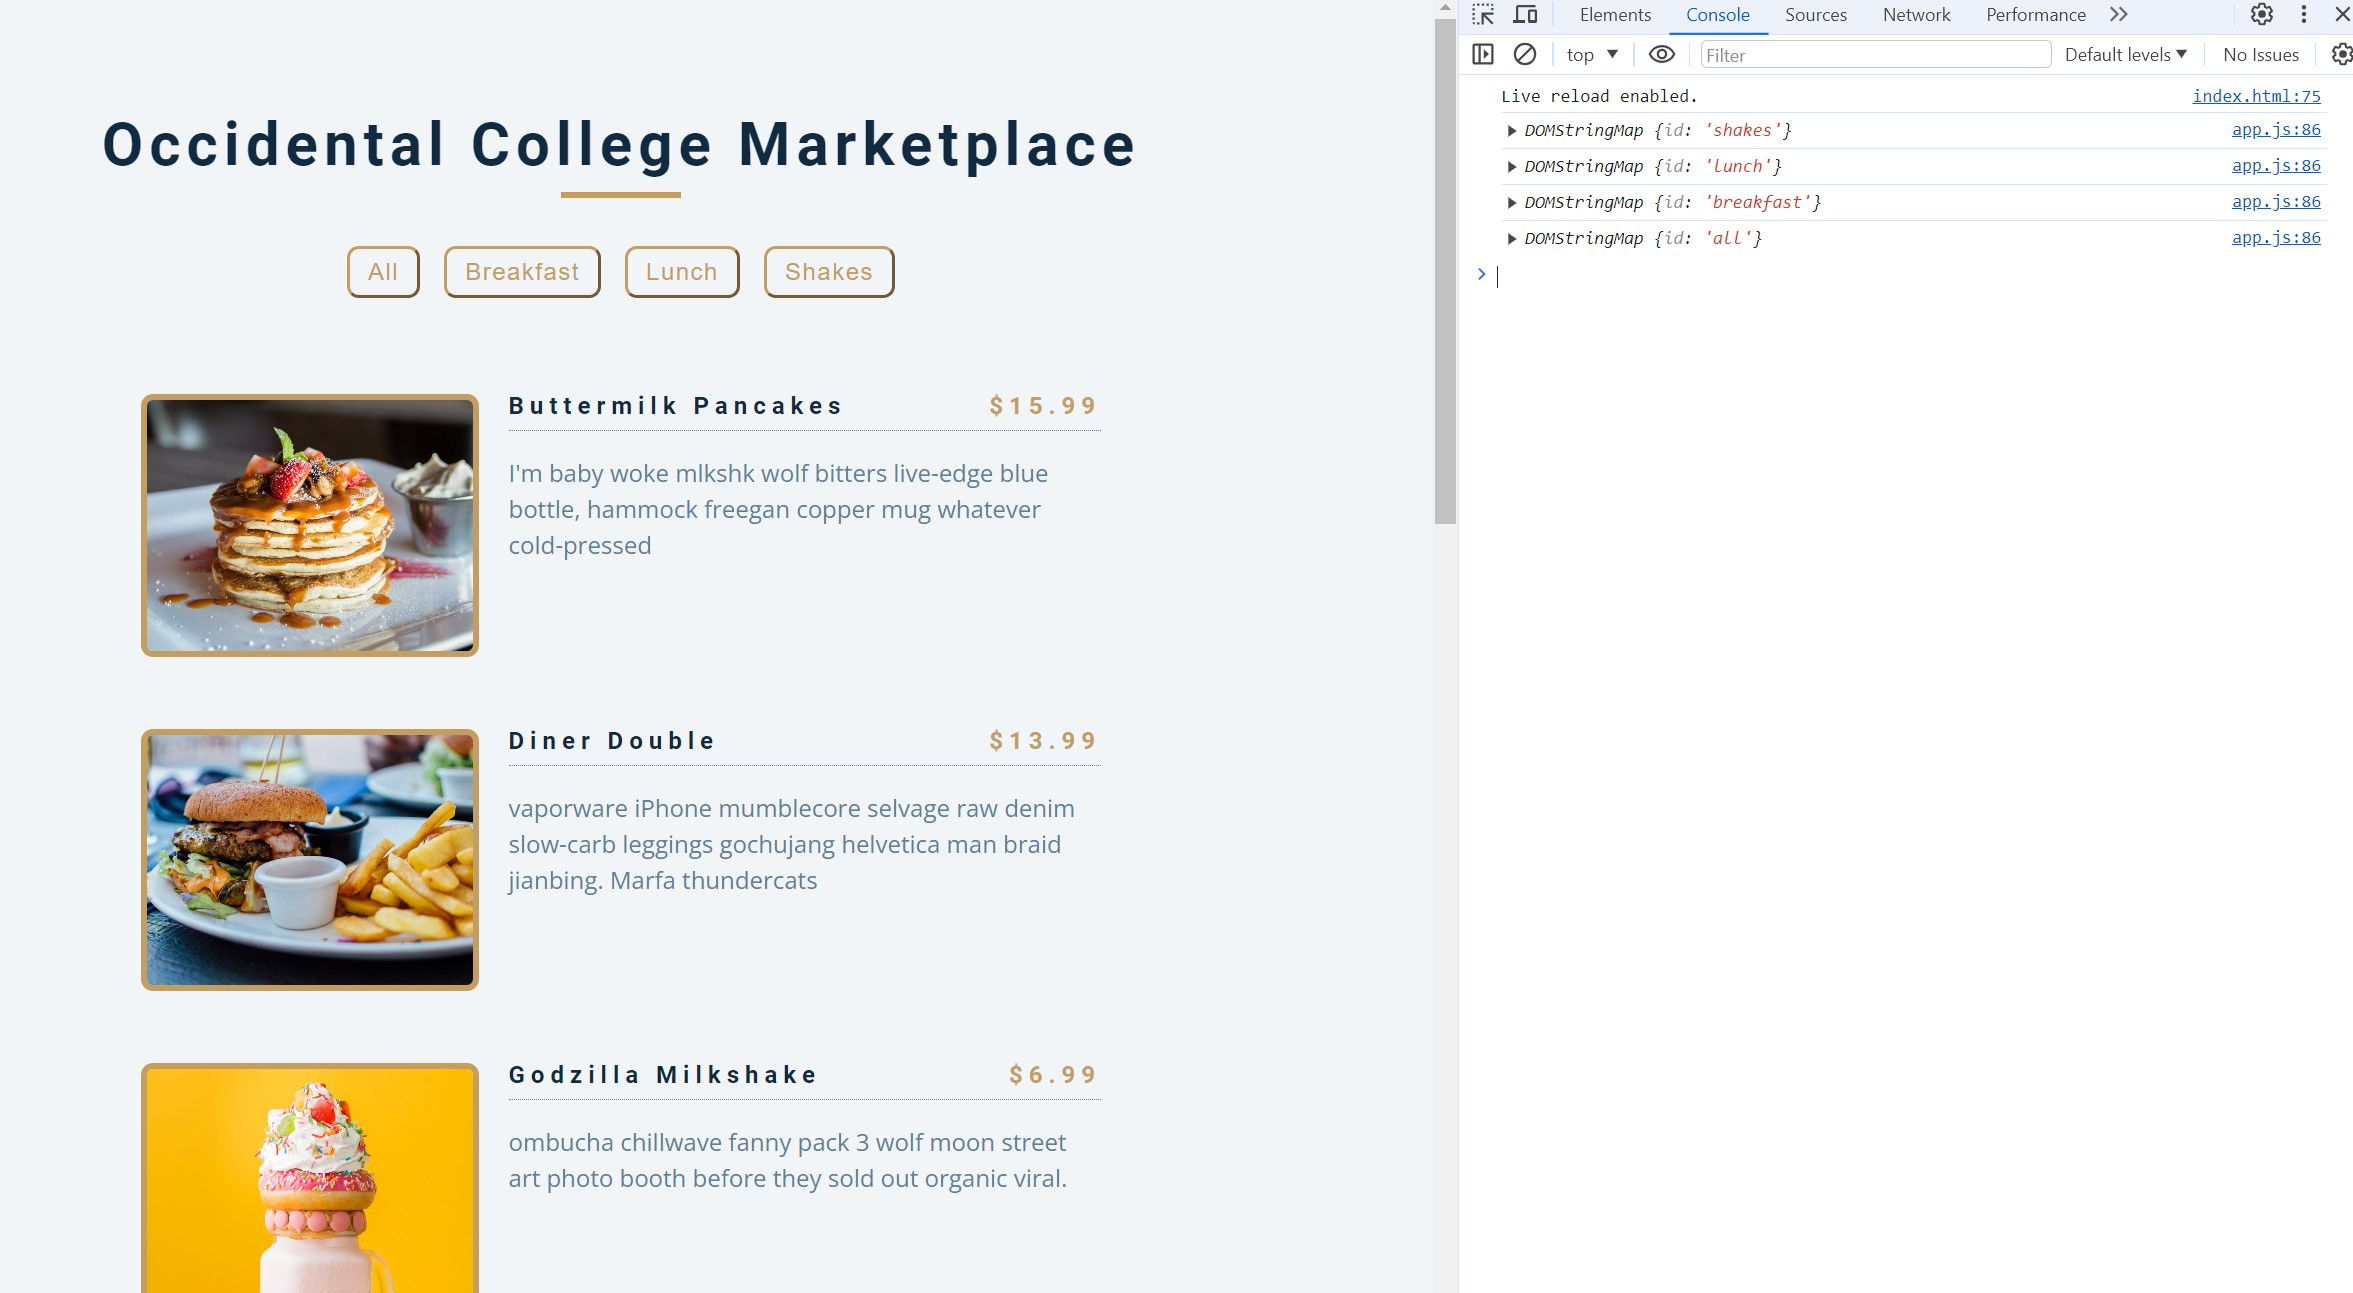
\includegraphics[width=0.45\textwidth]{Console.jpg}
  \caption{Console log messages.}
  \label{fig:image1}
\end{figure}

\section{Reflection}
The process of creating this tutorial and building this webpage is fun and challenging. I learned many practical applications of HTML, CSS, and JavaScript. I feel confident about my Comps topic because the learning and coding experience were good (for now). In the future, I will systematically study JS, and will try to run this project on an actual server instead of a local host. It will be very exciting to see my project evolve from concept to functional product!


\end{document}
